\section{Quick introduction to tensor and tensor field}
\begin{enumerate}[(I)]
    \item Let \(V\) be a vector space, \(\dim V=n\).
    \(V^*\) be the covector space=\{all linear functionals 
    \(\alpha\colon V\to \mathbb{R}\)\}. The pairing is given by 
    \[V^*\times V\to \mathbb{R}\]
    \[(\alpha,v)\mapsto \alpha(v)\]
    \begin{itemize}
        \item A \textcolor{blue}{covariant \(l\)-tensor} on \(V\)
        is a multilinear map 
        \textcolor{blue}{
            \[
                \omega\colon V\times \ldots \times V\to \mathbb{R}.
                \tag{1}    
            \]
        }
        A \textcolor{blue}{
            contravariant \(k\)-tensor 
        }
        is a multilinear map 
        \textcolor{blue}{
            \[
                X\colon V^*\times \ldots \times V^*\to \mathbb{R}.
                \tag{2}    
            \]
        }
        A \textcolor{blue}{
            tensor of \((k,l)\) type (\(k\)-contravariant, \(l\)-covariant)
        }
        is a multilinear map 
        \textcolor{blue}{
            \[
                T\colon  V^*\times \ldots \times V^*\times 
                V\times \ldots \times V \to \mathbb{R}.
                \tag{3}   
            \]
        }
        Let 
        \begin{center}
            \(
            \bigotimes^l V^*=\{\text{all covariant }l\text{-tensors}\}
            \Rightarrow \omega \text{ in (1) }\in \bigotimes^l V^*    
        \)

        \(
            \bigotimes^k V=\{\text{all contravariant }k\text{-tensors}\}
            \Rightarrow X \text{ in (2) }\in \bigotimes^k V    
        \)

        \(
            \mathcal{T}^{(k,l)}(V)=\{\text{all }(k,l)\text{-type tensors}\}
            \Rightarrow T\in \mathcal{T}^{(k,l)}(V)    
        \)
        \end{center}
        \item Next we talk about the \textcolor{blue}{tensor product}.
        Let \(T\in \mathcal{T}^{(k,l)}(V)\),
        \(S\in \mathcal{T}^{(p,q)}(V)\), then \(T\otimes S \in 
        \mathcal{T}^{(k+p,l+q)}(V)\) is defined as
        \textcolor{blue}{
            \begin{align*}
                &T\otimes S\left(\omega^1,\ldots,\omega^{k+p}
                ;X_1,\ldots, X_{l+q}\right)\\
                =&
                T\left(\omega^1,\ldots,\omega^{k}
                ;X_1,\ldots, X_{l}\right)
                S\left(\omega^{k+1},\ldots,\omega^{k+p}
                ;X_{l+1},\ldots, X_{l+q}\right) .
            \end{align*}
        } 
Let \(V=\Span\{E_1,\ldots,E_n\}\),
\(V^*=\Span\{\alpha^1,\ldots, \alpha^n\}\) with 
\(\alpha^i (E_j)=\delta^i_j\), or equivalently
\(E_j(\alpha^i)=\delta^i_j\). 

Then 
\[(1)\Rightarrow \omega=\omega_{i_1,i_2,\ldots,i_l} \alpha^{i_1}
\otimes \ldots \otimes \alpha^{i_l}.\]
Moreover, \begin{align*}
    \omega\left(E_{j_1},\ldots,E_{j_l}\right)
    &= \omega_{i_1,i_2,\ldots,i_l} \alpha^{i_1}
    \otimes \ldots \otimes \alpha^{i_l}\left(
        E_{j_1}\otimes \ldots\otimes E_{j_l}
    \right)\\
    &=\omega_{i_1,i_2,\ldots,i_l}
    \alpha^{i_1}(E_{j_1})\cdots \alpha^{i_l}(E_{j_l})\\
    &=\omega_{i_1,i_2,\ldots,i_l}\delta^{i_1}_{j_1}\cdots 
    \delta^{i_l}_{j_l}=\omega_{j_1\ldots j_l}.
\end{align*}
\[
    (2)\Rightarrow X=X^{i_1\ldots i_k} E_{i_1}\otimes \ldots 
    E_{i_k}.
\]
\[
    (3)\Rightarrow T=\tensor{T}{^{i_1\ldots i_k}_{j_1\ldots j_l}}
    E_{i_1}\otimes \ldots E_{i_k}\otimes \alpha^{j_1}\otimes 
    \ldots \otimes \alpha^{j_l} 
    \footnotemark
\]
\footnotetext{Tensor is ordered!}
    \end{itemize}
    \item On manifold \(M\), we have introduced 
    \begin{itemize}
        \item \(TM=\coprod_{p\in M} T_p M\) the tangent bundle. 
        \item \(T^*M=\coprod_{p\in M}T^*_p M\) cotangent bundle.
    \end{itemize}
    Now, we define \textcolor{blue}{
        \((k,l)\)-tensor bundle
        \[
            \mathcal{T}^{(k,l)}M=\coprod_{p\in M}\mathcal{T}^{(k,l)}_p M,    
        \]
    }
where \(\mathcal{T}^{(k,l)}_p M\) is the space of all \((k,l)\)-tensors
on \(T_p M\).
\textcolor{blue}{A tensor field \(T\) is a smooth map
\[
    T\colon M\to  \mathcal{T}^{(k,l)}M   
\]
\[
    p\mapsto T_p\in \mathcal{T}^{(k,l)}_p M.    
\]}
Let \((x^1,\ldots,x^n)\) be a local coordinate, then 
\[
    T=\tensor*{T}{^{i_1\ldots i_k}_{j_1\ldots j_l}} 
    \pdv{x^{i_1}}\otimes \ldots \otimes \pdv{x^{i_k}}
    \otimes d x^{j_1} \otimes \ldots \otimes d x^{j_l}.  
\]
\textcolor{pink}{
    {\Large \textbf{!}} \(T\left(\alpha^1,\ldots,\alpha^k;
    X_1,\ldots,X_l\right)\) is \(C^\infty\)-linear in each variable 
    \(\alpha^i\) and \(X_j\).
}
\end{enumerate}
\section{Induced Riemannian metric}
\begin{itemize}
    \item Let \((M,g)\) be a Riemannian manifold. Let \(p\in M\),
    and around \(p\) we have a local coordinate \((x^1,\ldots,x^n)\)
    \item \(T_p M=\Span\left\{
        \pdv{x^1},\ldots,\pdv{x^n}
    \right\}\), \(T^*_p M=\Span\left\{
        dx^1,\ldots,dx^n
    \right\}\).
    Moreover, 
    \textcolor{blue}{
        \[
            d x^i\left(\pdv{x^j}\right)=\delta^i_j.    
        \]
    }
    \item The Riemannian metric at \(p\) is
    \textcolor{blue}{
        \[
        g_p\colon T_p M\times T_p M\to \mathbb{R}    
        \]
        \[
            (V,W)\mapsto g_p(V,W)    
        \]
    }
    For a non-zero vector \(V\in T_p M\), this induces a linear map
    \[  
        \varphi_V\colon T_p M\to \mathbb{R}
        \]
\[W\mapsto \varphi_V(W)\]
\ie\ \(\vphi_V\in T^*_p M\)=\{all linear functionals on \(T_p M\)\}.
In particular, let \(V=\pdv{x^i}\), \(\forall W=\pdv{x^j}\)
\[
    \vphi_{\pdv{x^i}}\left(\pdv{x^j}\right)=g\left(\pdv{x^i},
    \pdv{x^j}\right)=g_{ij}.    
\]
Hence, as an element in \(T^*_p M\), we can write
\textcolor{blue}{
    \[\vphi_{\pdv{x^i}}=g_{ij}d x^j.\]
}
\item Discussions above says that we have a linear isomorphism
\[\vphi \colon T_p M\to T^*_p M\]
\[V\mapsto \vphi_V\]
\item Let \(\psi\colon T^*_p M\to T_p M\) be the inverse of \(\vphi\),
then 
\[
    T_p M \overset{\vphi}{\longrightarrow}T^*_p M\overset{\psi}{
        \longrightarrow
    }
    T_p M    
\]
\[
    \pdv{x^i}\mapsto g_{ij}d x^j\mapsto \pdv{x^i}    
\]
\ie\ \(\psi\left(g_{ij}d x^j\right)=g_{ij}\psi\left(d x^j\right)
=\pdv{x^i}\Rightarrow \psi\left(d x^j\right)=\textcolor{blue}{
    \underbracket{g^{ij}}_{\mathclap{\text{inverse of }(g_{ij})}}}
\pdv{x^i}\).

Moreover, for any covector \(\alpha=\alpha_j dx^j\)
\[
    \psi\left(\alpha_j dx^j\right)=\alpha_j g^{ij}\pdv{x^i}    
\]
\textcolor{blue}{
    \begin{definition}
        \begin{enumerate}[(1)]
            \item \[\vphi\colon T_p M\to T^*_p M\]
            \[v\mapsto\vphi(v)=\left(v^ig_{ij}\right)d x^j\]
            is called index-lowered down, usually denoted by 
            \(\vphi(v)=v_\flat\).\footnote{\(\flat\) for ``flat'' in music.}
            \item \[\psi\colon T^*_p M\to T_p M\]
            \[
                \alpha\mapsto \psi(\alpha)=\left(\alpha_i g^{ij}\right)
                \pdv{x^j}    
            \]
            is called index-lifted up, denoted by \(\psi(\alpha)
            =\alpha^{\sharp}\).\footnote{\(\sharp\) for ``sharp'' in music}
        \end{enumerate}
    \end{definition}
}
\item The linear isomorphism \(\sharp\) enables us to extend the Riemannian
metric on \(T^* M\), \ie\ \(\forall p\in M\)
\textcolor{blue}{
    \[
        \tilde{g}\colon T^*_p M\times T^*_p M\to\mathbb{R}    
    \]
    \[
        (\alpha,\beta)\mapsto \tilde{g}(\alpha,\beta)    
    \]
}
such that
\textcolor{blue}{
    \[
        \tilde{g}(\alpha,\beta):=g\left(\alpha^\sharp,\beta^\sharp\right)    .
    \]
}
In local coordinate, \(\alpha=\alpha_i dx^i,\beta=\beta_j dx^j\)
\begin{align*}
    \tilde{g}(\alpha,\beta)&= g\left(\alpha_i g^{ik}\pdv{x^k}
    ,\beta_j g^{jl}\pdv{x^l}\right)=\alpha_i g^{ik}\beta_j g^{jl}g
    \left(\pdv{x^k},\pdv{x^l}\right)\\
    &=\alpha_i g^{ik}\beta_j \underbrace{g^{jl}g_{kl}}_{\delta^j_k}
    =\alpha_i\beta_j g^{ij}.
\end{align*}
\ie\ \textcolor{blue}{
    \(\tilde{g}(\alpha,\beta)=g^{ij}\alpha_i\beta_j\)}.
In particular, \(\tilde{g}\left(dx^i,dx^j\right)=g^{ij}\). 

In general, we can extend the Riemannian metric to any tensor of the same
type, \ie\ 
\textcolor{blue}{
    \(\forall S, T\) are two \(p,q\) tensors, locally
    \[
        S=\tensor*{S}{^{i_1\ldots i_p}_{j_1\ldots j_q}}
        \pdv{x^{i_1}}\otimes \ldots \otimes\pdv{x^{i_p}}\otimes 
        dx^{j_1}\otimes\ldots \otimes dx^{j_q}.    
    \]
    \[
        T=\tensor*{T}{^{i_1\ldots i_p}_{j_1\ldots j_q}}
        \pdv{x^{i_1}}\otimes \ldots \otimes\pdv{x^{i_p}}\otimes 
        dx^{j_1}\otimes\ldots \otimes dx^{j_q}.    
    \]
    Then \(\tilde{g}(S,T):=\tensor*{S}{^{i_1\ldots i_p}_{j_1\ldots j_q}}
    \tensor*{T}{^{k_1\ldots k_p}_{l_1\ldots l_q}} g_{i_1k_1}g_{i_2k_2}
    \cdots g_{i_p k_p} g^{j_1 l_1}\cdots g^{j_q l_q}\).
}
\end{itemize}
\begin{example}
    \begin{enumerate}[(1)]
        \item If \(S=S_{ij}dx^i\otimes dx^j\), \(T=T_{pq}dx^p\otimes dx^q\),
        then
        \[
            \tilde{g}(S,T)=S_{ij}T_{pq}g^{ip}g^{jq}.    
        \]
        \item \(\nabla f= df =f_i d x^i\),
        \(\mathrm{grad} f= g^{ij} f_j \pdv{x^i}\).
        \[
            \begin{rcases}
                \Rightarrow &\left|\nabla f\right|^2 =
                g\left(f_i dx^i,f_j dx^j\right)=g^{ij} f_i f_j.\\
                &\left|\mathrm{grad} f\right|^2= g^{ij} f_j g^{kl}f_l g_{ik}
                =g^{ij}f_i f_j.
            \end{rcases}
            \Rightarrow
            |\nabla f|^2=|\mathrm{grad} f|^2.  
        \]
        \item From (1), \(\mathrm{Hess} f =\nabla_i\nabla_j f dx^i\otimes
        d x^j\),
        \footnote{Recall that \(\nabla_i\nabla_j f=\pdv{f}{x^i}{x^j}
        -\Gamma\indices*{_{ij}^k}\pdv{f}{x^k}\).}
        \[\Rightarrow |\mathrm{Hess} f|^2= g^{ik}g^{jl}\nabla_i\nabla_j f
        \nabla_k\nabla_l f.\]
    \end{enumerate}
\end{example}
\section{Bochner formula in 2-dimensional Riemannian manifold}
\textcolor{red}{
    \begin{theorem}
        Let \((S,g)\) be a 2-dimensional Riemannian manifold,
        \(f\in C^3(S)\), then
        \[
            \frac{1}{2}\Delta |\nabla f|^2 =|\nabla\nabla f|^2+\left\langle
                \nabla\left(\Delta f\right),\nabla f\right\rangle 
                +K|\nabla f|^2.   
        \]
    \end{theorem}
}
\textcolor{teal}{
    \begin{remark}
        \begin{enumerate}[(1)]
            \item In your homework, you have shown that on the
            Euclidean space
            \[\frac{1}{2}\Delta |\nabla f|^2 =|\nabla\nabla f|^2+\left\langle
                \nabla\left(\Delta f\right),\nabla f\right\rangle. \]
            \item On a general Riemannian manifold, the Bochner formula
            is
            \textcolor{red}{
                \[\frac{1}{2}\Delta |\nabla f|^2 =|\nabla\nabla f|^2+
                \left\langle\nabla\left(\Delta f\right),
                \nabla f\right\rangle 
                +\mathrm{Ric}(\nabla f,\nabla f).\]
            }
        \end{enumerate}
    \end{remark}
}
\begin{proof}
    \begin{align*}
        \Delta |\nabla f|^2
        &=g^{ij}\nabla_i\nabla_j \left(g^{kl}\nabla_k f\nabla_l f\right)\\
        &=g^{ij}g^{kl}\left(
            \nabla_i\nabla_j\nabla_k f\nabla_l f+ \nabla_i\nabla_j\nabla_l f
            \nabla_k f+\nabla_i\nabla_l f\nabla_j \nabla_k f
            +\nabla_i\nabla_k f\nabla_j\nabla_l f \right)\\
        &=2 g^{ij}g^{kl}\nabla_i\textcolor{blue}{\nabla_j\nabla_k f}
            \nabla_l f+ 2 g^{ij}g^{kl}\nabla_i\nabla_k f\nabla_j\nabla_l f\\
        &=2|\nabla\nabla f|^2 + 2 g^{ij}g^{kl}\nabla_i 
        \textcolor{blue}{\nabla_k\nabla_j f}\nabla_l f.
    \end{align*}
    To further compute R.H.S., we take
    \textcolor{teal}{geodesic polar coordinate
    \[
        ds^2=dr^2+G(r,\theta)d\theta^2\Rightarrow g^{-1}=\begin{pmatrix}
            1&0\\
            0& \frac{1}{G}
        \end{pmatrix}.    
    \]
    }
    \begin{align*}
        &g^{ij}g^{kl}\nabla_i\nabla_k\nabla_j f\cdot \nabla_l f
        =g^{kl}\nabla_i\nabla_k\nabla^i f\nabla_l f\\
        =&\nabla_i\nabla_1\nabla^i f\cdot \nabla_1 f
        +\frac{1}{G}\nabla_i\nabla_2\nabla^i f\nabla_2 f\\
        =&\nabla_1\nabla_1\nabla^1 f \cdot \nabla_1 f+\nabla_2 \nabla_1
        \nabla^2 f\cdot \nabla_1 f+\frac{1}{G}\left(
            \nabla_1\nabla_2\nabla^1 f\nabla_2 f+\nabla_2\nabla_2\nabla^2 f
            \nabla_2 f
        \right)
    \end{align*}
    \begin{enumerate}[(1)]
        \item \begin{align*}
            \nabla_2\nabla_1\left(\nabla^2 f\right)\cdot \nabla_1 f
            &=\nabla_1 \nabla_2 \left(\nabla^2 f\right)\cdot + 
            \tensor{R}{_{21}^2_i}\nabla^i f\nabla_1 f
            \\
            &=\nabla_1 \nabla_2 \left(\nabla^2 f\right)\cdot \nabla_1 f
            + R_{212i}g^{22}\nabla^i f\nabla_1 f \\
            &=\nabla_1 \nabla_2 \nabla^2 f\cdot \nabla_1 f
            +R_{2121}\frac{1}{G}\nabla^1 f\nabla_1 f.
        \end{align*}
        \item \begin{align*}
            \nabla_1 \nabla_2 \nabla^1 f\cdot \nabla_2 f
            &=\nabla_2 \nabla_1 \nabla^1 f\cdot \nabla_2 f+ 
            \tensor{R}{_{12}^1_i}\nabla^i f \nabla_2 f\\
            &=\nabla_2\nabla_1 \nabla^1 f\cdot \nabla_2 f
            +R_{1212}\nabla^2 f\nabla_2 f.
        \end{align*}
    \end{enumerate}
    Note that \(R_{1212}=R_{2121}\) and \(K=\dfrac{R_{1212}}{G}\).
        \begin{align*}
            & g^{kl}\nabla_i\nabla_k\nabla^i f
            \cdot \nabla_l f\\
            =&\underbracket{\nabla_1\nabla_1\nabla^1 f
            \nabla_1 f+ \nabla_1\nabla_2\nabla^2 f \nabla_1 f 
            }_{(1)}+\underbracket{K\nabla^1 f\nabla_1 f}_{(2)}\\
            &
            +\underbracket{\frac{1}{G}\left(
                \nabla_2\nabla_1\nabla^1 f \nabla_2 f
                +\nabla_2\nabla_2\nabla^2 f \nabla_2 f
            \right)}_{(1)}+\underbracket{K\nabla^2 f\nabla_2 f}_{(2)}\\
            =&\nabla_1\left(\Delta f\right)\nabla_1 f
            +\frac{1}{G}\left(\nabla_2(\Delta f)\nabla_2 f\right)
            + K|\nabla f|^2\\
            =&\left\langle\nabla(\Delta f),\nabla f\right\rangle
            +K |\nabla f|^2.
        \end{align*}
        Hence, \(
            \frac{1}{2}\Delta |\nabla f|^2 =|\nabla\nabla f|^2+\left\langle
                \nabla\left(\Delta f\right),\nabla f\right\rangle 
                +K|\nabla f|^2    
        \).
\end{proof}
To obtain interesting geometry results, it(Bochner formula) needs to combine with
analysis tools, one of such tools is the following maximum principle.
\begin{theorem}[Hopf-Calabi: Maximum principle]
    \hfill
    \begin{itemize}
        \item \((M,g)\) is a connected Riemannian manifold.
        \item \(f\colon M\to \mathbb{R}\): \(C^\infty\) subharmonic function,
        \ie\ \(\Delta_g f\ge 0\).
    \end{itemize}
    \(\Rightarrow\)\(f\) attains no maximum unless it's constant.
\end{theorem}
The proof is based on the standard maximum principle in the P.D.E.
theory. We'll show, if \(f\) attains maximum at \(p\in M\), then \(f\)
must be a constant. (Again, we'll consider the \(\dim M=2\) case
in the following, and in higher dimension arguments are similar.)
    \begin{enumerate}[\textbf{Step} 1]
        \item (Strong version) If \(\Delta f>0\), then \(f\) has no local
        maximum.
        \begin{proof}
            If \(f\) attains local max at \(p\in M\), then
            \(\nabla f(p)=0\) and \(\nabla\nabla f\le 0\Rightarrow
            \Delta f(p)\le 0\).
        \end{proof}
        \item (Weak version) If \(\Delta f\ge 0\), and \(f\) attains global
        maximum at \(p\), then f is constant.
        \begin{proof}(By perturbation method)
            If \(f\) attains global maximum at \(p\), then \(p\) is also a 
            local maximum of \(f\). Assume \(f\) is not a constant in any
            neighborhood of \(p\), then we may choose a sufficient
            small coordinate ball(geodesic ball) \(B\) of \(p\)
            such that
            \[
                S=\{x\in \partial B |f(x)\ge f(p)-1\}
                \footnotemark
            \]
            \footnotetext{This is modified slightly by the TA.}
            (You can choose 1 here after replacing \(f\) by some \(\lambda 
            f\))
            is a proper subset of \(\partial B\) (\ie\ there must be some
            \(\bar{q} \in \partial B\), \(f(\bar{q})< f(p)\)).
            \begin{center}
                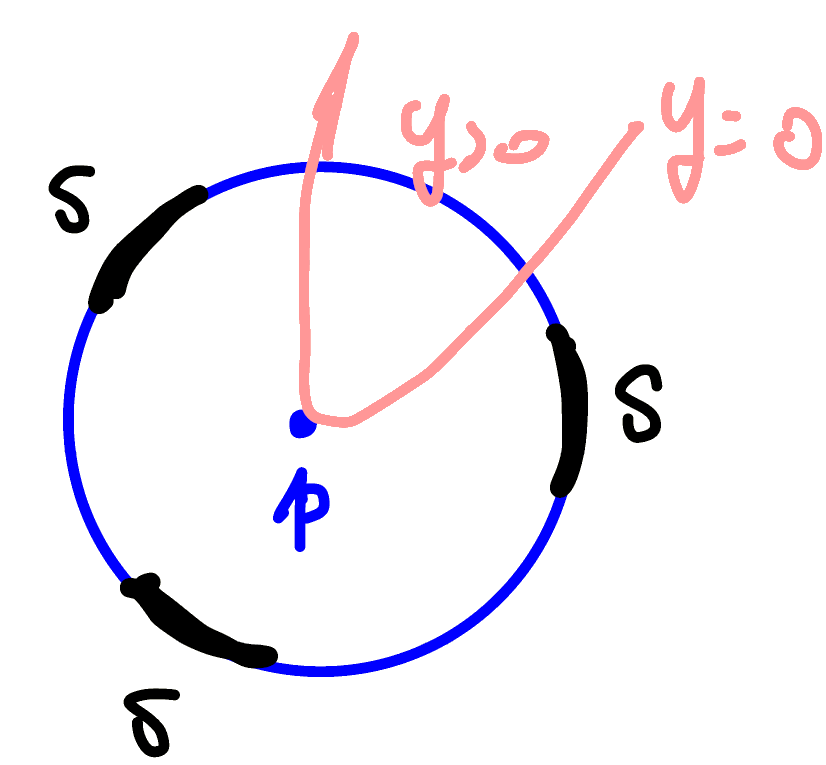
\includegraphics[scale=0.4]{
                    picture/week13/maximum principle.png}
            \end{center}
            By a suitable choice of coordinate \((x,y)\), we can further
            assume \(p\) lies on \(y=0\) and \(S\) lies on \(\{y<0\}\).
            Consider coordinate \(y(q)\) for \(\forall q\in B_p(r)\),
            then \(y\) is a smooth function on \(\bar{B}\).
            
            Note that
            \begin{enumerate}[(1)]
                \item \(y(p)=0\), and \(y<0\) on \(S\).
                \item \(|\nabla y|^2=|g^{22}|\neq 0\)(By
                positive-definiteness).
                \item \(|\Delta y|=|g^{ij}\Gamma\indices*{_{ij}^2}|
                \le A\) for some constant \(A>0\).
            \end{enumerate}
            Let \(h=e^{cy}-1\) for \(c\gg 1\), then
            \begin{enumerate}[(1)]
                \item \(h(p)=0\).
                \item \(\Delta h=c e^{cy}\left(c|\nabla y|^2\right)+
                \Delta y\). Note that \(|\Delta y|\le A\),
                \(|\nabla y|\neq 0\), we
                can choose \(c\) sufficiently large such that
                \[
                    \Delta h>0 \text{ on } \bar{B}.    
                \]
                \item \(h<0\) on \(S\).
            \end{enumerate}
Now consider a perturbation of \(f\)
\[
    f_\epsilon=f+\epsilon h,0<\epsilon\ll 1.
\]
Then
\begin{enumerate}[(1)]
    \item \(f_\epsilon(p)=f(p)+\epsilon h(p)=f(p)\).
    \item \(\Delta f_\epsilon=\Delta f+\epsilon \Delta h>0\) on \(\bar{B}\).
    \item \(f_\epsilon\) must attain maximum inside \(B\). Since
    \(\forall x\in \partial B\), if \(x\) lies in \(S=\{x|f(x)\ge f(p)-1\}\),
    note that \(p\) is a local maximum, and \(S\subset \{y<0\}\), then 
    \[f_\epsilon< f_\epsilon(p) \text{ on }S.\]
    If \(x\in \partial B- S\), \ie\ \(f(x)< f(p)-1\), take \(\epsilon\)
    sufficiently small such that \(|\epsilon h(x)|<1\) on \(\partial B\),
    then one has 
    \[f_\epsilon(x)<f_\epsilon(p) \text{ on }\partial B-S.\]
    This contradicts the strong maximum principle.
\end{enumerate}
\end{proof}
\end{enumerate}
\begin{exercise}[Maximum principle in 1-dimensional calculus]
    Show that
    \begin{enumerate}[(1)]
        \item \(x\in \mathbb{R}\), \(f''(x)>0\), then \(f\) has no upper
        bound.
        \item \(x\in \mathbb{R}\), \(f''(x)\ge 0\), if
        \(\exists x_0\in\mathbb{R}\) such that \(f(x_0)=A=\max f(x)\),
        then \(f(x)=A\) for all \(x\in \mathbb{R}\).
    \end{enumerate}
\end{exercise}
\section{Induced covariant derivative on tensor fields}
Let \(\nabla\) be the Levi0Civita connection on \((M,g)\), then for 
\(\forall\) vector field \(X\in \Gamma(TM)\), the covariant derivative
\(\nabla_X\) is 
\[
    \nabla_X\colon \Gamma(TM)\to \Gamma(TM)    
\]
\[
    Y\mapsto \nabla_X Y    
\]
and locally 
\[
    \nabla_{\pdv{x^i}}\pdv{x^j}=\Gamma\indices*{_{ij}^k}\pdv{x^k}.    
\]
Since \(T^* M\) is the dual bundle of \(TM\), we can extend \(\nabla_X\)
on \(T^*M\) as 
\[
    \nabla_X\colon \Gamma(T^*M)\to \Gamma(T^*M)    
\]
\[
    \omega\mapsto  \nabla_X \omega  
\]
such that \(\forall Y\in \Gamma(TM)\)
\[
    \left(\nabla_X \omega\right)(Y)
    =\nabla_X\left(\omega(Y)\right)-\omega\left(\nabla_X Y\right).
\]
Locally, \(\Gamma(T^*M)=\Span\{dx^1,\ldots,dx^n\}\)
\begin{align*}
    \left(\nabla_{\pdv{x^i}}d x^j\right)\left(\pdv{x^k}\right)
    &=\nabla_{\pdv{x^i}}\left(d x^j \left(\pdv{x^k}\right)\right)-
    d x^j\left(\nabla_{\pdv{x^i}}\pdv{x^k}\right)\\
    &=- dx^j\left(\Gamma\indices*{_{ik}^ p}\pdv{x^p}\right)\\
    &=-\Gamma\indices*{_{ik}^j}.
\end{align*}
\(\Rightarrow \boxed{
    \nabla_{\pdv{x^i}}d x^j =-\Gamma\indices*{_{ik}^j} dx^k
}\).
Now, let \(T\) be a \(p,q\)-tensor
\[
    T=\tensor*{T}{^{i_1\ldots i_p}_{j_1\ldots j_q}}
        \pdv{x^{i_1}}\otimes \ldots \otimes\pdv{x^{i_p}}\otimes 
        dx^{j_1}\otimes\ldots \otimes dx^{j_q}.    
\]
Then
\begin{align*}
    \nabla_k T&=\nabla_k \left(
        \tensor*{T}{^{i_1\ldots i_p}_{j_1\ldots j_q}}
        \pdv{x^{i_1}}\otimes \ldots \otimes\pdv{x^{i_p}}\otimes 
        dx^{j_1}\otimes\ldots \otimes dx^{j_q}
        \right)\\
        &=\partial_k \tensor*{T}{^{i_1\ldots i_p}_{j_1\ldots j_q}}
        \pdv{x^{i_1}}\otimes \ldots \otimes\pdv{x^{i_p}}\otimes 
        dx^{j_1}\otimes\ldots \otimes dx^{j_q}\\
        &\phantom{=}+\sum_{\alpha=1}^p
        \tensor*{T}{^{i_1\ldots i_\alpha\ldots i_p}_{j_1\ldots j_q}}
        \pdv{x^{i_1}}\otimes \ldots \otimes
        \nabla_k\left(\pdv{x^i_{\alpha}}\right)\otimes
        \ldots \otimes\pdv{x^{i_p}}\otimes 
        dx^{j_1}\otimes\ldots \otimes dx^{j_q}\\
        &\phantom{=}+\sum_{\beta=1}^q
        \tensor*{T}{^{i_1\ldots i_p}_{j_1\ldots j_\beta \ldots j_q}}
        \pdv{x^{i_1}}\otimes \ldots \otimes\pdv{x^{i_p}}\otimes 
        dx^{j_1}\otimes\ldots\otimes \nabla_k\left(
        d x^{j_\beta}\right)\otimes\ldots \otimes dx^{j_q}\\
        &=\partial_k \tensor*{T}{^{i_1\ldots i_p}_{j_1\ldots j_q}}
        \pdv{x^{i_1}}\otimes \ldots \otimes\pdv{x^{i_p}}\otimes 
        dx^{j_1}\otimes\ldots \otimes dx^{j_q}\\
        &\phantom{=}+\sum_{\alpha=1}^p
        \tensor*{T}{^{i_1\ldots \gamma\ldots i_p}_{j_1\ldots j_q}}
        \Gamma\indices*{_{k\gamma}^{i_\alpha}}
        \pdv{x^{i_1}}\otimes \ldots\otimes\pdv{x^{i_p}}\otimes 
        dx^{j_1}\otimes\ldots \otimes dx^{j_q}\\
        &\phantom{=}-\sum_{\beta=1}^q 
        \tensor*{T}{^{i_1\ldots i_p}_{j_1\ldots\theta \ldots j_q}}
        \Gamma\indices*{_{kj_\beta}^\theta}
        \pdv{x^{i_1}}\otimes \ldots \otimes\pdv{x^{i_p}}\otimes 
        dx^{j_1}\otimes\ldots \otimes dx^{j_q}.
\end{align*}
\begin{align*}
    \therefore\nabla_k T&=\left(
    \partial_k \tensor*{T}{^{i_1\ldots i_p}_{j_1\ldots j_q}}
    +\sum_{\alpha=1}^p
    \tensor*{T}{^{i_1\ldots \gamma\ldots i_p}_{j_1\ldots j_q}}
    \Gamma\indices*{_{k\gamma}^{i_\alpha}}\right.\\
    &\phantom{aaaaaaaaaaa}\left.
    -\sum_{\beta=1}^q 
        \tensor*{T}{^{i_1\ldots i_p}_{j_1\ldots\theta \ldots j_q}}
        \Gamma\indices*{_{kj_\beta}^\theta}
    \right)\pdv{x^{i_1}}\otimes \ldots \otimes\pdv{x^{i_p}}\otimes 
    dx^{j_1}\otimes\ldots \otimes dx^{j_q},
\end{align*}
or
\[\nabla_k \tensor*{T}{^{i_1\ldots i_p}_{j_1\ldots j_q}}
=\partial_k \tensor*{T}{^{i_1\ldots i_p}_{j_1\ldots j_q}}
+\sum_{\alpha=1}^p
\tensor*{T}{^{i_1\ldots \gamma\ldots i_p}_{j_1\ldots j_q}}
\Gamma\indices*{_{k\gamma}^{i_\alpha}}
-\sum_{\beta=1}^q 
\tensor*{T}{^{i_1\ldots i_p}_{j_1\ldots\theta \ldots j_q}}
\Gamma\indices*{_{kj_\beta}^\theta}\]